\documentclass{article}
\usepackage[utf8]{inputenc}
\usepackage{graphicx}
	\DeclareGraphicsExtensions{.png, .jpeg}
\usepackage{caption}
% \usepackage{subcaption}
\usepackage{csvsimple}
\usepackage[top=1in, bottom=1in, left=1in, right=1in]{geometry}

\title{PA04: Vector Reduce Revisited\\CS791v: Parallel Computing}
\author{Terence Henriod}
\date{\today}

\begin{document}

\clearpage
\maketitle
\thispagestyle{empty} % removes the page number from the title page

\begin{abstract}
In this assignment, we revisit vector reduction techniques on the GPU, this time attempting an array of techniques instead of just one. The first is vector reduction via kernel calls from the CPU; the second is reduction using a in itial kernel to pre-sum the elements followed by a final reduction kernel launch from within the original kernel; third is using the GPU to initially reduce the vector to an intermediate vector, and then complete the summation on the CPU; the final version is to use the \texttt{threadfence} instruction to have one block perform the final summation of the intermediate vector.
\end{abstract}

\newpage
\section{Introduction}
Vector reduction is a common, highly parallelizable task. It also provides ample flexibility to explore different GPU techniques in a simplified way. Even though reduction is typically summarized as simply ``summing all of the elements of a vector," the addition operation can be substituted to adapt reduction to a variety of tasks. Since elements can be operated on in any order, and only need to be operated only once, 

\section{Theory}
Here we discuss the methodologies of the various methods.

\subsection{Reduction Through Multiple Kernel Launches}
The most ``naive" way to reduce a vector. A kernel is used to task blocks with reducing the original vector into an intermediate vector that has as many elements as there were blocks in the kernel launch. In order to complete the reduction, the intermediate vector needs to be reduced once all of the blocks have completed their task. Since inter-block synchronization is difficult and costly to implement on hardware, the programmer can effect the inter-block synchronization by simply making a second kernel call that uses a single block to reduce the intermediate vector to a single element.

\subsection{Reduction Through Kernels That Launch Kernels}
Possibly the most ``brute force" way to accomplish this is to perform a vector reduction, then call a similar reduction with fewer blocks, and continue in this manner until the resulting intemediate vector is a favorable size for reduction into a single block by a final kernel launch (this is the method that was implemented). This can be slightly awkward, and requires a form of inter-block synchronization.

Perhaps a more elegant way that I did not think of until I was already writing this report would be to divide the vector appropriately, make recursive calls to process those vector segments, continue breaking the vector down to a favorable size, and then combining the results as the recursion recedes back up the ``tree." This would have been far more interesting to explore, but there was not the time to implement it. This would still require synchronization between blocks after the child calls have completed, which is a problem that is not easily solved (and generally isn't on GPUs, except via splitting up kernel launches).

\subsection{Reduction With a Kernel Launch and Final Reduction on the CPU}
While the GPU can provide large speedups through its massive parallelism, GPU kernels have high start-up and tear down costs, not to mention the need for memory transfers. Because of this, it can be beneficial to have smaller tasks be completed on the CPU. This way the CPU's quickness can be applied without large startup costs or memory transfers. In vector reduction, this takes the form of having the CPU perform the final reduce on the intermediate vector.

\subsection{Reduction With a Single Kernel and Inter-Block Synchronization}
As mentioned previously, inter-block synchronization is costly to implement, and so it is not done. Mostly. There is a special thread synchronization function known as \texttt{threadfence}. This instruction allows GPU code to make guarantees about the order of some operations. Using the \texttt{threadfence}, a vector can be reduced to an intermediate vector, then the fence can synchronize operations, and then the intermediate vector can be passed to a single block for final reduction.

\newpage
\section{Results}
The performance results of the various vector reduction methods are displayed here. A note about the line graphs: the times were so close that it may be difficult to separate the different methods. I apologize, but I did not want to fill this report with SPAM graphs. We only want HAM graphs.

\subsection{Information on the GPU device used}
\csvautotabular{gpu_properties.csv}

\newpage
\subsection{Performance Graphs}
  \begin{figure}[h!]
    \centering
    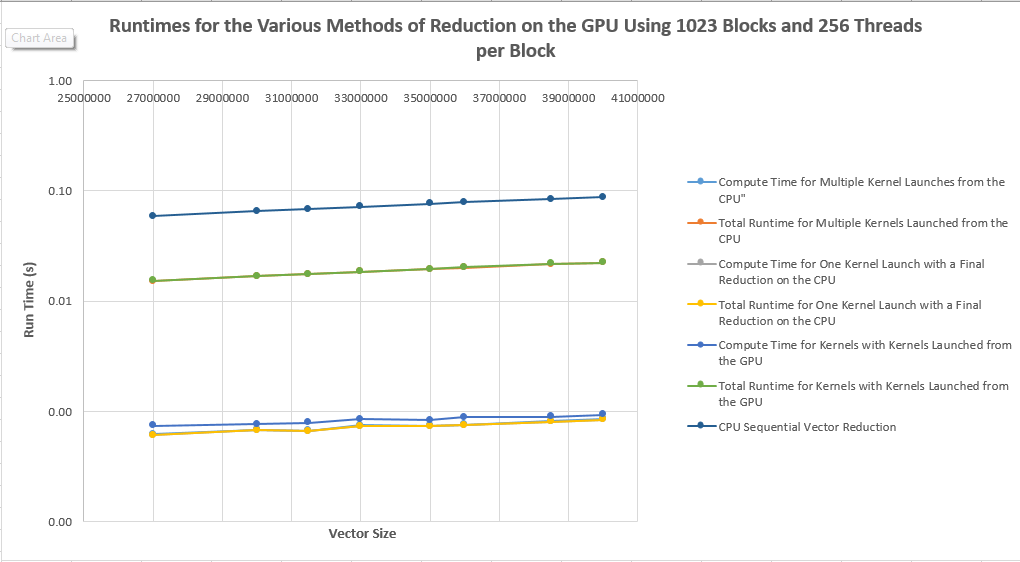
\includegraphics[width=.9\linewidth]{runtime_line}
    \caption{A comparison of the runtimes for reduction across vectors of various sizes.}
    \label{fig:runtime_line}
  \end{figure}

  \begin{figure}[h!]
    \centering
    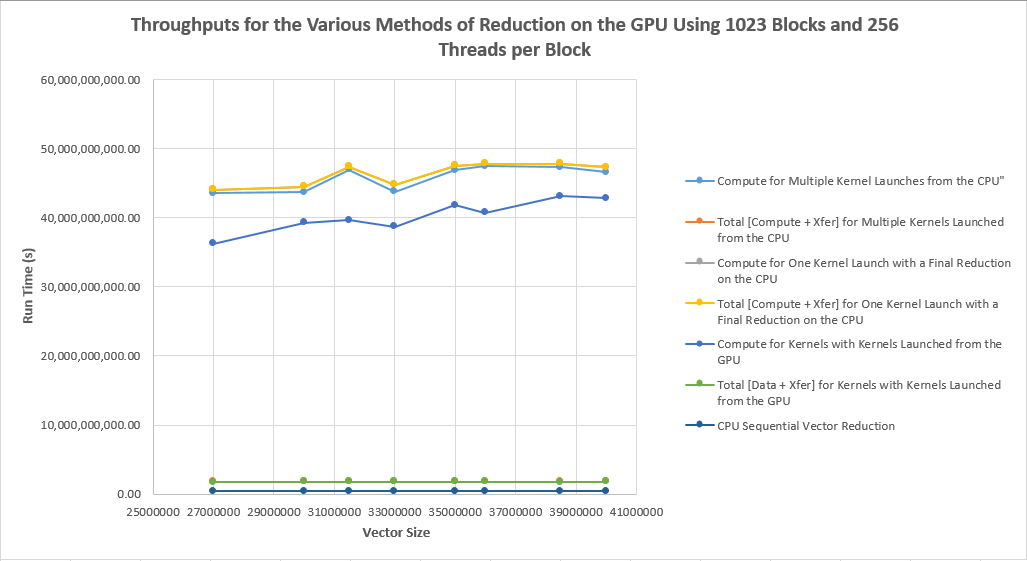
\includegraphics[width=.9\linewidth]{throughput_line}
    \caption{A comparison of the throughput for vector reduction of various sizes.}
    \label{fig:throughput_line}
  \end{figure}

  \begin{figure}[h!]
    \centering
    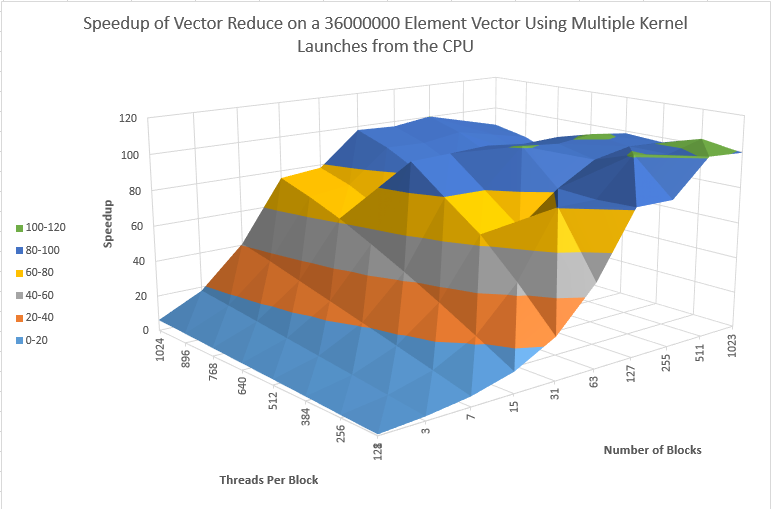
\includegraphics[width=.9\linewidth]{multi_kernel_surface}
    \caption{The speedup achieved using multiple kernel launches for a representative vector size.}
    \label{fig:multi_kernel_surface}
  \end{figure}

  \begin{figure}[h!]
    \centering
    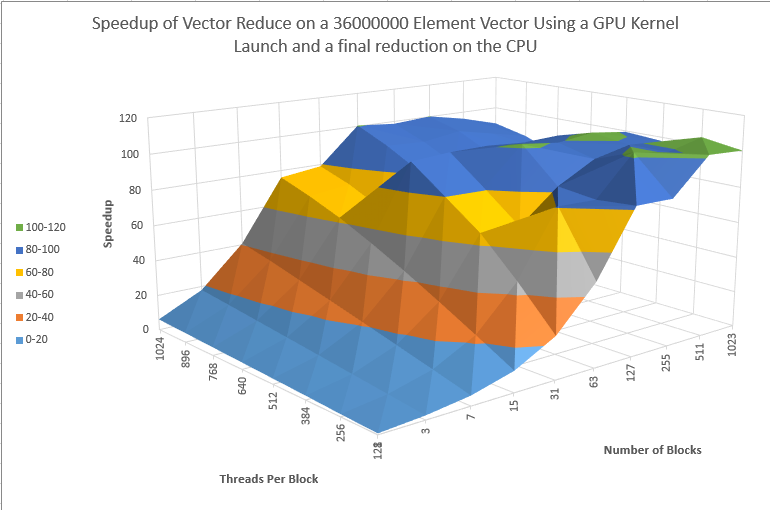
\includegraphics[width=.9\linewidth]{cpu_finish_surface}
    \caption{The speedup achieved when reducing the vector with the GPU and then performing the final reduction on the CPU for a representative vector size.}
    \label{fig:cpu_finish_surface}
  \end{figure}

  \begin{figure}[h!]
    \centering
    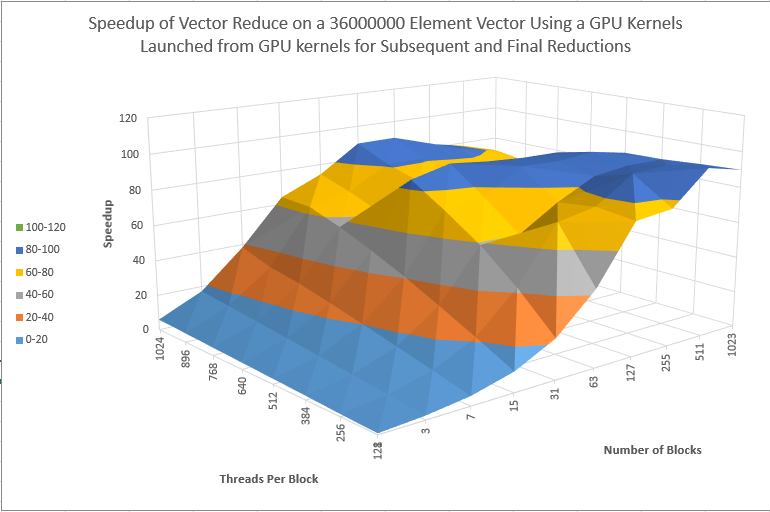
\includegraphics[width=.7\linewidth]{kernel_in_kernel_surface}
    \caption{The speedup of the ``GPU Recursive" method for a vector of representative size.}
    \label{fig:kernel_in_kernel_surface}
  \end{figure}

\newpage
\section{Discussion}
\subsection{Blocks and Threads}
It was apparent that a smaller number of threads, but not too small (around 256 per block) was ideal as far s threads were concerned. I would be willing to wager that the reason higher numbers of threads prevent larger speedups is because they oversaturate the SMs. With several warps (like in the 256 thread case), threads that need to access memory will have some latency to hide while the data is fetched. A good number of warps will hide this latency, without leaving warps that have already had their data fetched waiting. It seems that for the GeForce GTX 780, 8 warps per block is ideal.

However, it appears that numbers of blocks only improve performance as they increase. This is very likely due to the fact that larger numbers of blocks reduce the vectors faster and will require fewer steps/kernel launches/etc. to completely reduce the vector.

\subsection{Many Kernel Launches vs. Final Reduction on the CPU}
These two methods were surprisingly close, and according to the results, when larger block sizes are used, the CPU finisher version performed slightly better. This is likley due to the fact that the larger block-sized kernels reduce to a small enough intermediate vector that the CPU can handle it more easily than at other sizes. However, if there had been time to handle extremely large sizes, I am curious to see if the CPU finisher's relative performance would drop again.

\subsection{Kernel Recursion vs. The Others}
After hearing some of the rumors of the GPUs poor performance with recursion (such as a limit on call depth of 25 and general slow performance), I was surprised to see that the recursive method was still able to achieve $70-80\%$ of the speedup of the other kernels. I am willing to bet that this is due largely to the fact that synchronization between blocks is still required. Since there is no good inter-block synchronization method available explicitly in CUDA, the programmer is left to improvise. The programmer must figure out a way to sychronize without deadlocking the system, which is very much non-trivial. Brute force or elegant method, I believe the weakness of the GPU at recursion/dynamic parallelism and inter-block synchronization. However, it did still provide large speedup over the sequential version, so there is potential there. I think though that the dynamic parallelism featture was designed to be used on problems that have a lot more data independence or it should be used in concert with the standard technique of issuing separate kernel launches from the CPU to achieve inter-block synchronization.

\subsection{Using \texttt{threadfence()} to Have a Final Block Perform the Final Reduction (or not)}
Unfortunately, due to needing to share computing resources with other students and already being so near the deadline, I was unable to attempt the extra credit algorithm. I think this could have been intersting to explore, especially if a technique such as this was properly paired with the recursive strategy.

\section{Issues}
\subsection{Unreliable Hardware}
I experienced a lot of difficulty with the machine that was used for this assignment. I used the machine in Dr. Harris HPVIS lab that had the only GPU capable of dynamic parallelism to complete the assignment. I wrote and tested my other code using my laptop. The code ran reliably and without issue. However, one I ported the code to the other machine, suddenly using $2047$ blocks resulted in the ``Invalid configuration" CUDA error. I tried modifying the number of threads used, tried many numbers of blocks above and below the $1023$ mark, only to find that everything above $1023$ blocks was an invalid configuration. This is disappointing because judging by the speedup graphs, there is a possibility of more speedup when using more blocks. Without sufficient support, I was unable to find the cause of this failure and had to move on and limit my experiments to at most $1024$ blocks. Much to my chagrin, I could have used more blocks had my laptop been capable of dynamic parallelism.

Further, the GPU memory allocation was unreliable, where I was able to reliably allocate memory on my laptop, the lab machine would sometimes successfully allocate vectors as large as ~80 million, or sometimes fail around the 16 million mark. This was frustrating during data collection.

\subsection{The ``GPU Recursive" Algorithm}
With little direction on how to design the recursive algorithm, I initially went with the ``brute force" method described previously. This resulted in having to invent ways of synchronizing all of the blocks before the subsequent kernel launches. This was difficult since a \texttt{threadfence()} couldn't quite do the job. So I added counter that made use of a global variable to count the blocks as they finished. This meant having a ``master thread" that needed to spin-lock while waiting for this count-off to finish. The GPU is very unlikely to pre-empt a block that is waiting, which is somewhat unfortunate. However, I found that with some reliability, issuing a small print statement will in fact pre-empt the block and let others run, granting me success with a curious little hack.
  
\end{document}
